\chapter{Prílohy}
\label{chap:prilohy}

{\huge Namiesto vymenovavania ciest k suborom na CD to urobit tak, ze do kapitoly "Prilohy" dať cislovany zoznam tak, aby odzrkadloval hierarchicku adresarovu strukturu na CD. Potom sa iba odkazovať na casti v cislovanom zozname. Cislovany zoznam zacinat od cisla kapitoly}



\begin{enumerate}
  \setcounter{enumi}{10}
  \item fifth element
\end{enumerate}




CD médium obsahuje:

\begin{itemize}[noitemsep]
    \item Text bakalárskej práce,
    \item Návody na používanie pre virtualizačný nástroj
    \item Tabuľkový dokument so sumárnym vyhodnotením všetkých otestovaných zariadení pre virtualizačný nástroj spolu so všetkými meraniami,
    \item Tabuľkový dokument s prehľadom všetkých vyučovaných technológii na vybraných predmetoch a ich kompatibilitou s vybranými virtuálnymi zariadeniami,
    \item Integračný balíček EVE-ng pre platformy Windows a Linux.
\end{itemize}




\section{Používanie EVE-ng}

Pre zvolené predmety boli topológie vytvorené podľa toho, aká téma bola na danom cvičení vyučovaná. Topológie boli vytvorené pomocou webového rozhrania EVE-ng, ktorým je možné spravovať topológie a používateľov.




\subsection{Vytvorenie topológie}
\label{chap:vytvorenie_topo_eve-ng}
Predtým, než popíšeme výsledky pri nasadení na predmety, sa najprv budeme venovať vytváraniu topológii, ktoré nasadeniu predchádzali. Nižšie sú uvedené kroky na vytvorenie topológie v EVE-ng.

\begin{enumerate}[noitemsep]

    \item \label{item:prihlasenie} Najprv sa prihlásime do nástroja EVE-ng cez webové rozhranie v natívnom móde. Webové rozhranie je dostupné v 2 módoch: natívnom a HTML5 (obr. \ref{obr:eve_ng_login_screen}). Rozdiely medzi jednotlivými módmi sú popísané v bode \ref{item:vzdialeny_pristup}. Pre úspešné prihlásenie musíme mať vytvorený používateľský účet, čo môže urobiť iba používateľ s rolou \emph{admin}.

\begin{figure}
    \centering
    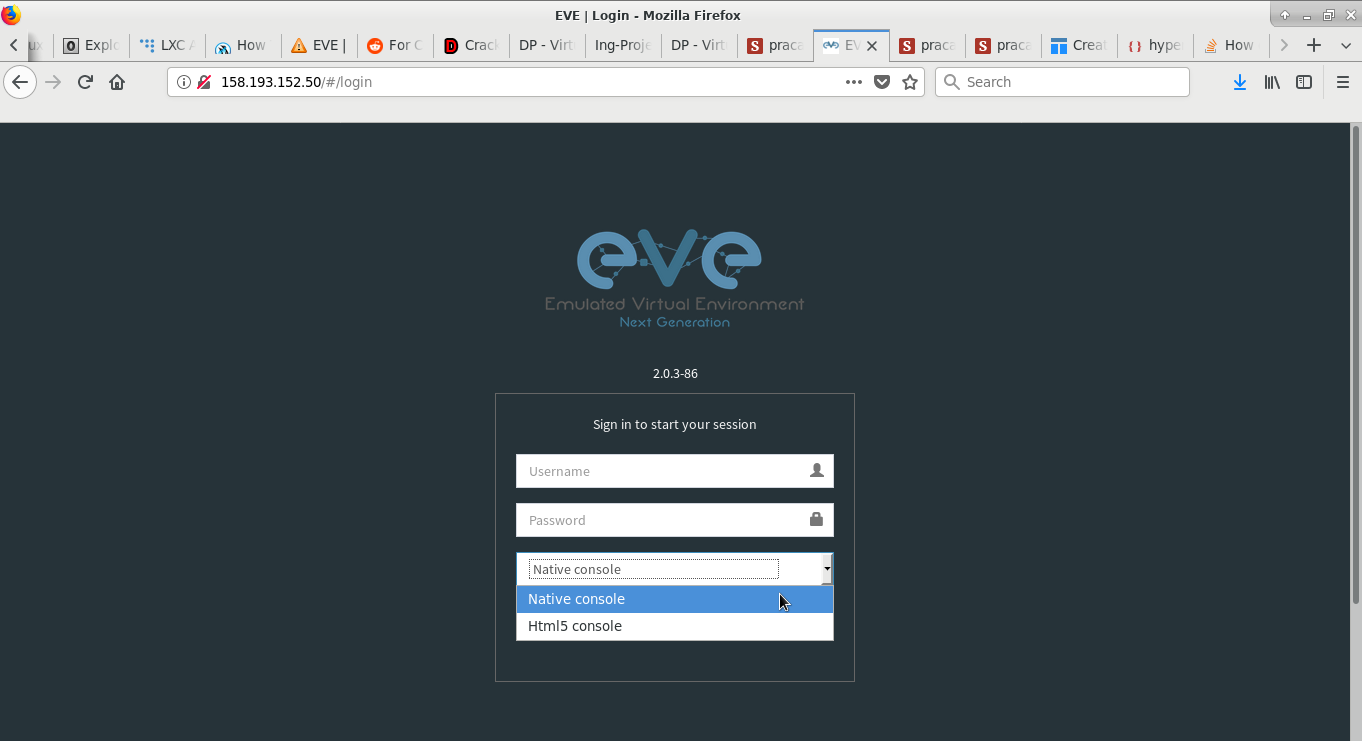
\includegraphics[width=0.75\textwidth]{eve_ng_login_screen}
    \caption{Prihlasovacia obrazovka EVE-ng}
    \label{obr:eve_ng_login_screen}
\end{figure}

    \item Po prihlásení sa zobrazí hlavná obrazovka (obr. \ref{obr:eve_ng_main_screen}). V ľavej časti je správca súborov, v ktorom si vyberieme adresár, kde bude uložený súbor s topológiou.

\begin{figure}
    \centering
    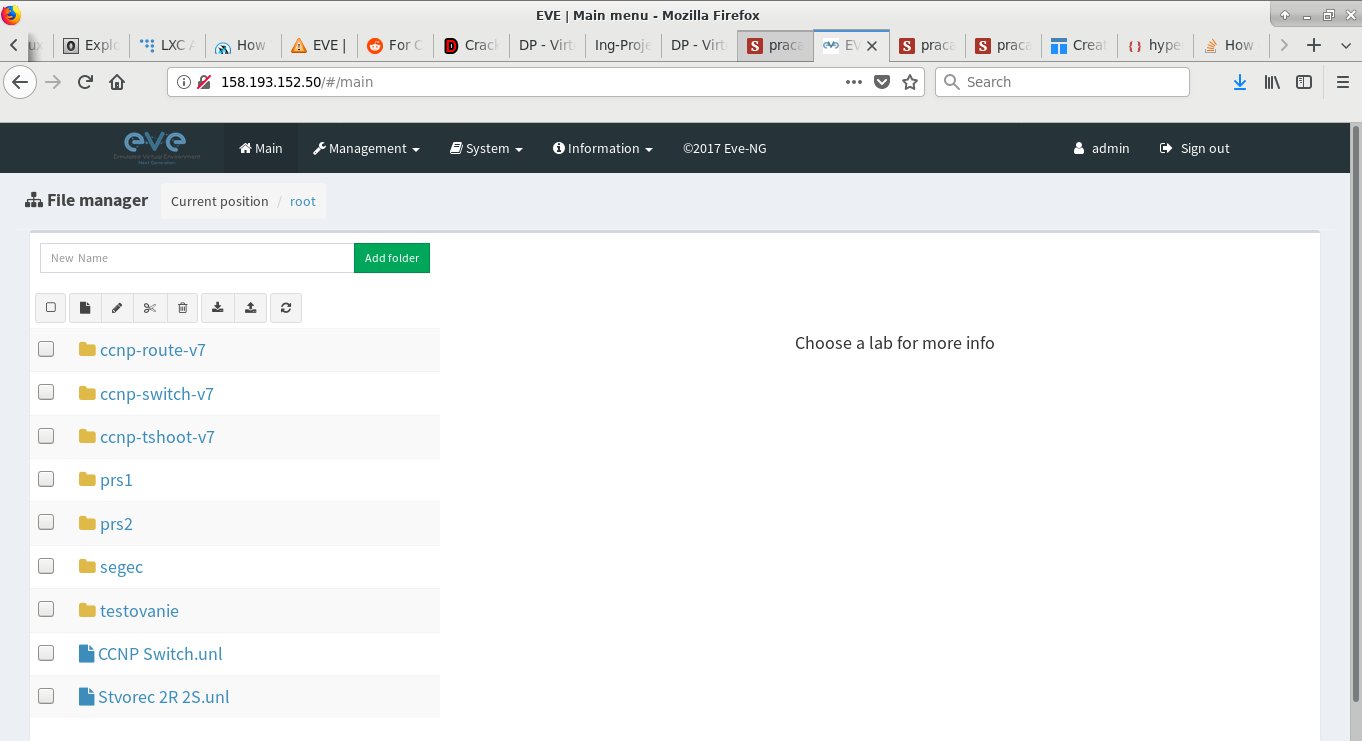
\includegraphics[width=0.75\textwidth]{eve_ng_main_screen}
    \caption{Hlavná obrazovka EVE-ng}
    \label{obr:eve_ng_main_screen}
\end{figure}

    \item Po výbere adresára klikneme na ikonku hárku s popisom \emph{Add new lab} (obr. \ref{obr:eve_ng_lab_menu}), čím začneme vytváranie novej topológie. Topológiu môže vytvoriť iba používateľ s rolou \emph{editor} alebo \emph{admin}.

\begin{figure}
    \centering
        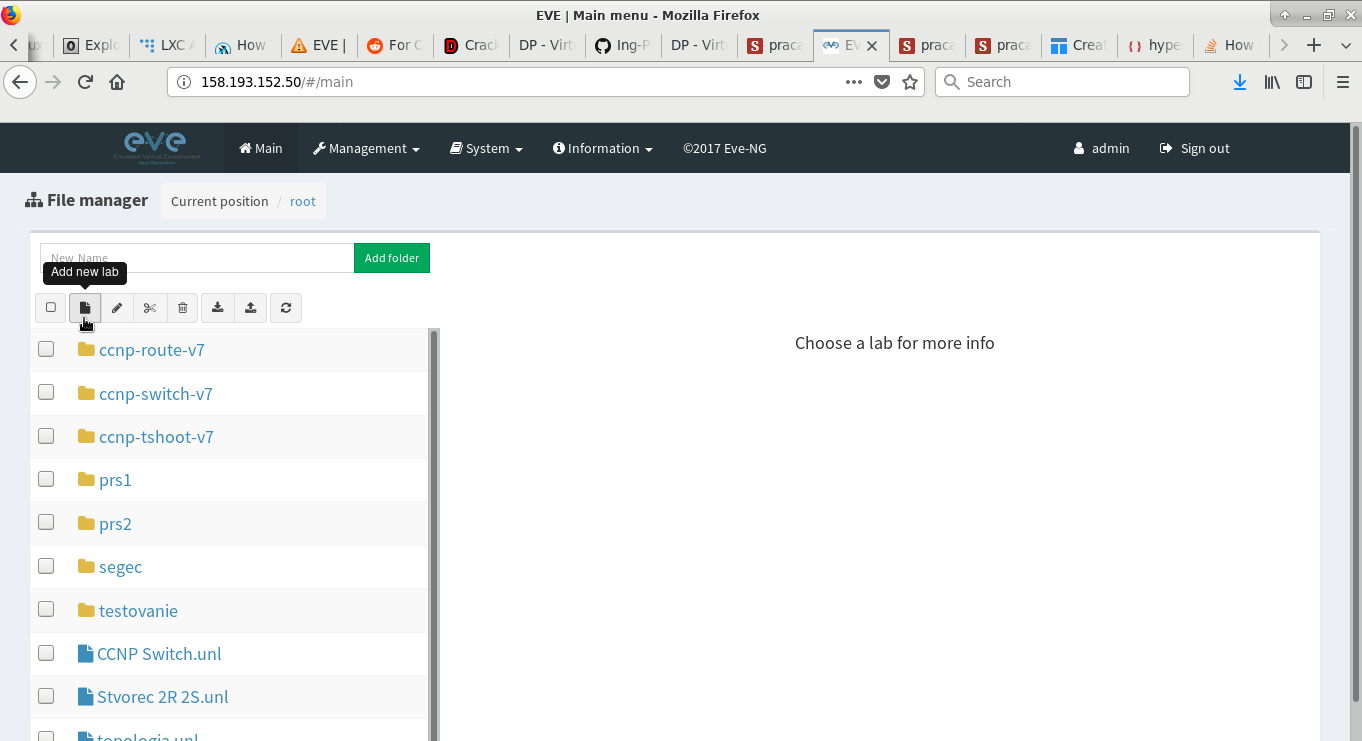
\includegraphics[width=0.75\textwidth]{eve_ng_lab_menu}
    \caption{Menu pre úpravu súborov}
    \label{obr:eve_ng_lab_menu}
\end{figure}

    \item Zobrazí sa dialógové okno, do ktorého zadáme atribúty topológie (obr. \ref{obr:eve_ng_lab_dialog}). Pre úspešné vytvorenie súboru stačí vyplniť iba povinné atribúty: \emph{Name} (názov topológie) a \emph{Version} (verzia topológie).

\begin{figure}
    \centering
    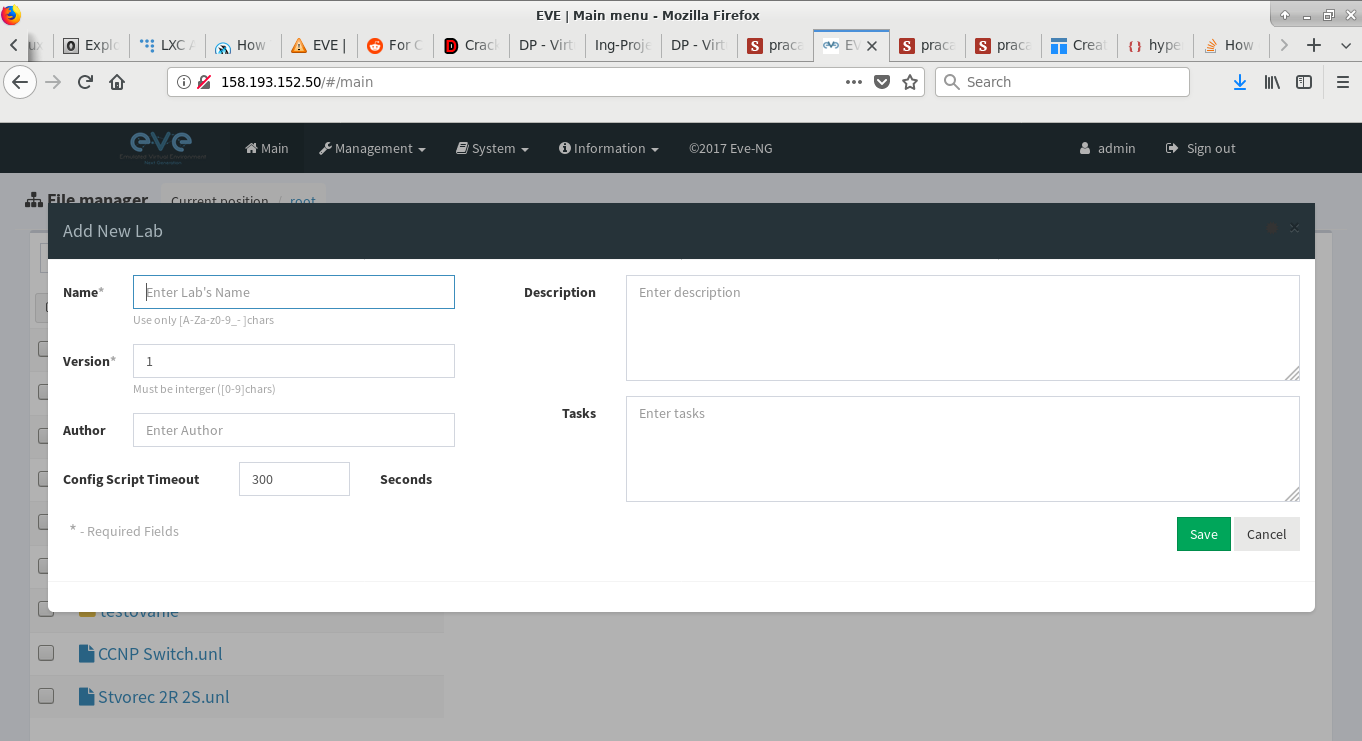
\includegraphics[width=0.75\textwidth]{eve_ng_lab_dialog}
    \caption{Dialógové okno na vytvorenie nového súboru s topológiou}
    \label{obr:eve_ng_lab_dialog}
\end{figure}

    \item Po kliknutí na tlačidlo \emph{Save} sa súbor s topológiou vytvorí a následne sa zobrazí pracovná plocha na vytvorenie topológie (obr. \ref{obr:eve_ng_nova_topologia}). Novovytvorená topológia  je prázdna.

\begin{figure}
    \centering
    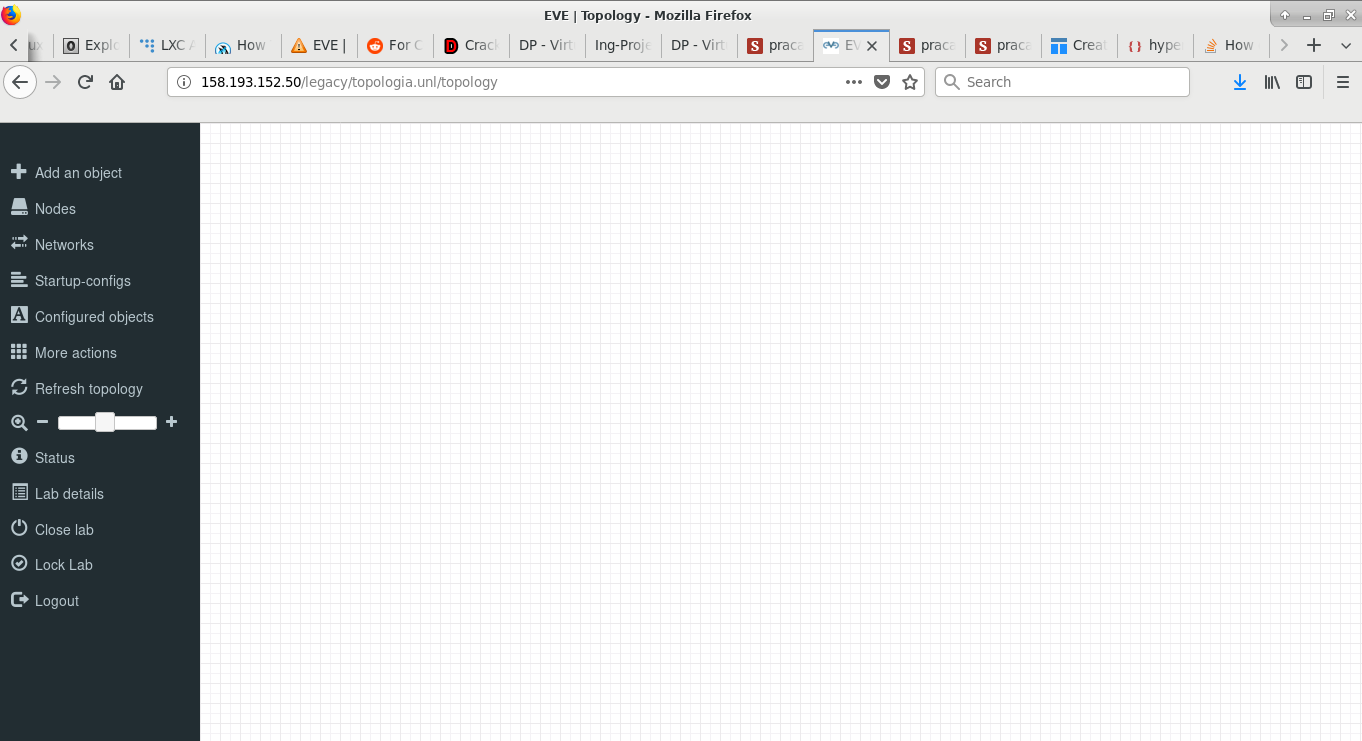
\includegraphics[width=0.75\textwidth]{eve_ng_nova_topologia}
    \caption{Ukážka novovytvorenej topológie}
    \label{obr:eve_ng_nova_topologia}
\end{figure}

    \item Do topológie môžeme po jej vytvorení pridávať tieto prvky:
    
    \begin{itemize}[noitemsep]
        \item Node - zariadenie
        \item Network - sieť
        \item Picture - obr.
        \item Custom Shape - geometrický tvar - obdĺžnik/elipsa
        \item Text - textové polia
    \end{itemize}
    
    Spomenutý zoznam prvkov (obr. \ref{obr:eve_ng_add_new_object_context_menu}) sa zobrazí v kontextovom menu po pravom kliknutí na prázdne miesto v topológii alebo po kliknutí na ikonku \emph{+} v menu na ľavej strane obrazovky. Po pridaní zariadenia výberom položky \emph{Node} sa pre zariadenie vygeneruje a priradí portové číslo, pomocou ktorého bude možné, pripojiť sa na jeho konzolu. Generovanie portových čísel pre zariadenia v EVE-ng je bližšie vysvetlené v časti \ref{chap:priradovanie_portovych_cisel} - \nameref{chap:priradovanie_portovych_cisel}.

\begin{figure}
    \centering
    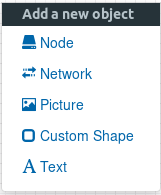
\includegraphics[width=0.75\textwidth]{eve_ng_add_new_object_context_menu}
    \caption{Kontextové menu pre pridanie zariadenia}
    \label{obr:eve_ng_add_new_object_context_menu}
\end{figure}
    
    \item Po pridaní prvkov do topológie vytvoríme spojenia medzi jednotlivými zariadeniami. Zariadenia je možné prepájať iba rozhraniami rovnakého typu (Ethernet-Ethernet, Serial-Serial). Prepájať je možné iba \emph{vypnuté} zariadenia. Prepojenie medzi zariadeniami vytvoríme kliknutím na ikonu \emph{vidlice} s popisom \emph{Connect to another node} (obr. \ref{obr:eve_ng_prepajanie_vidlica}) a potiahnutím myši smerom ku druhému zariadeniu (obr. \ref{obr:eve_ng_prepajanie_ku_druhemu_zariadeniu}). Následne sa objaví dialógové okno s výberom rozhraní pre obidve zariadenia, ktoré majú byť prepojené (obr. \ref{obr:eve_ng_prepajanie_add_connection_dialog}). Po výbere rozhraní z oboch rozbaľovacích zoznamov klikneme na tlačidlo \emph{Save}. Dialógové okno sa zatvorí a vytvorí sa prepojenie medzi zariadeniami pre zvolené rozhrania (obr. \ref{obr:eve_ng_prepajanie_prepojenie_vytvorenie}). Po nastavení správnych IP adries na prepojených rozhraniach bude vytvorená konektivita medzi zariadeniami.
    
    \begin{figure}
        \centering
        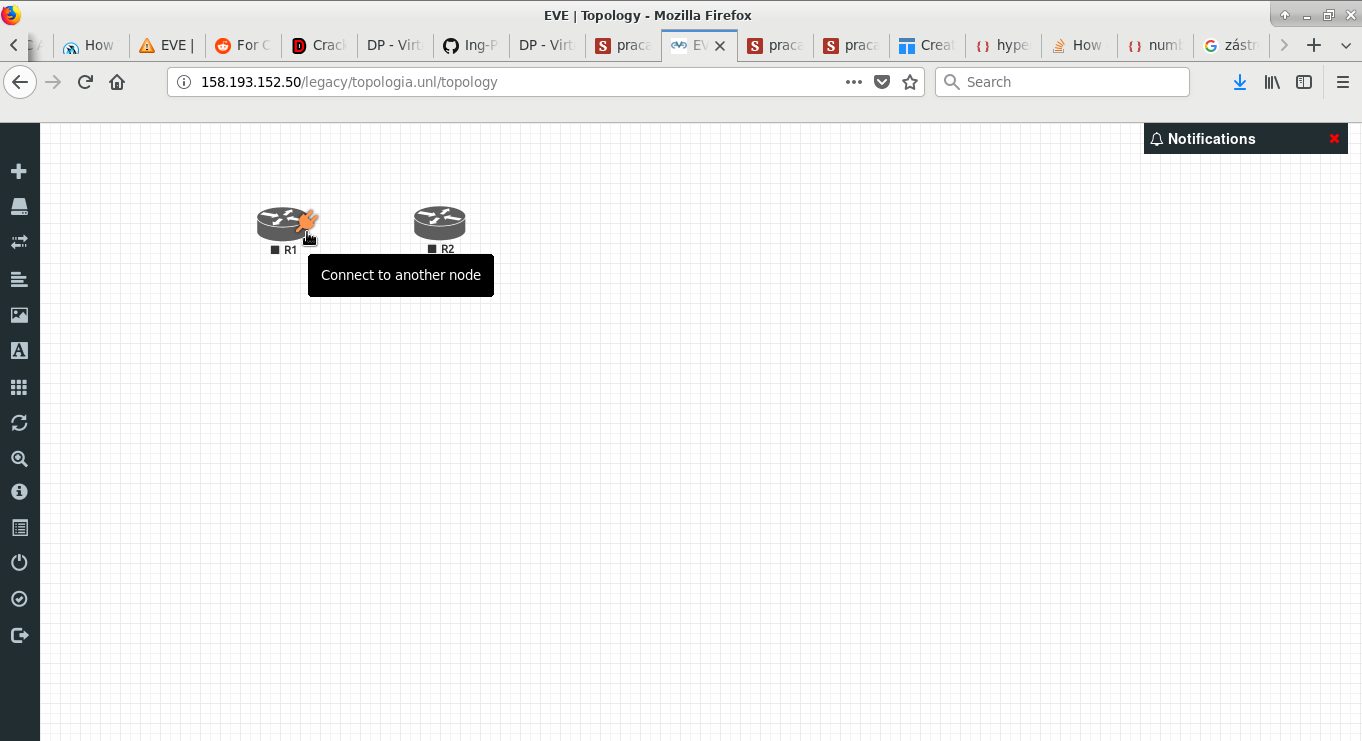
\includegraphics[width=0.75\textwidth]{eve_ng_prepajanie_vidlica}
        \caption{Ikona na prepájanie zariadení}
        \label{obr:eve_ng_prepajanie_vidlica}
    \end{figure}
    
    \begin{figure}
        \centering
        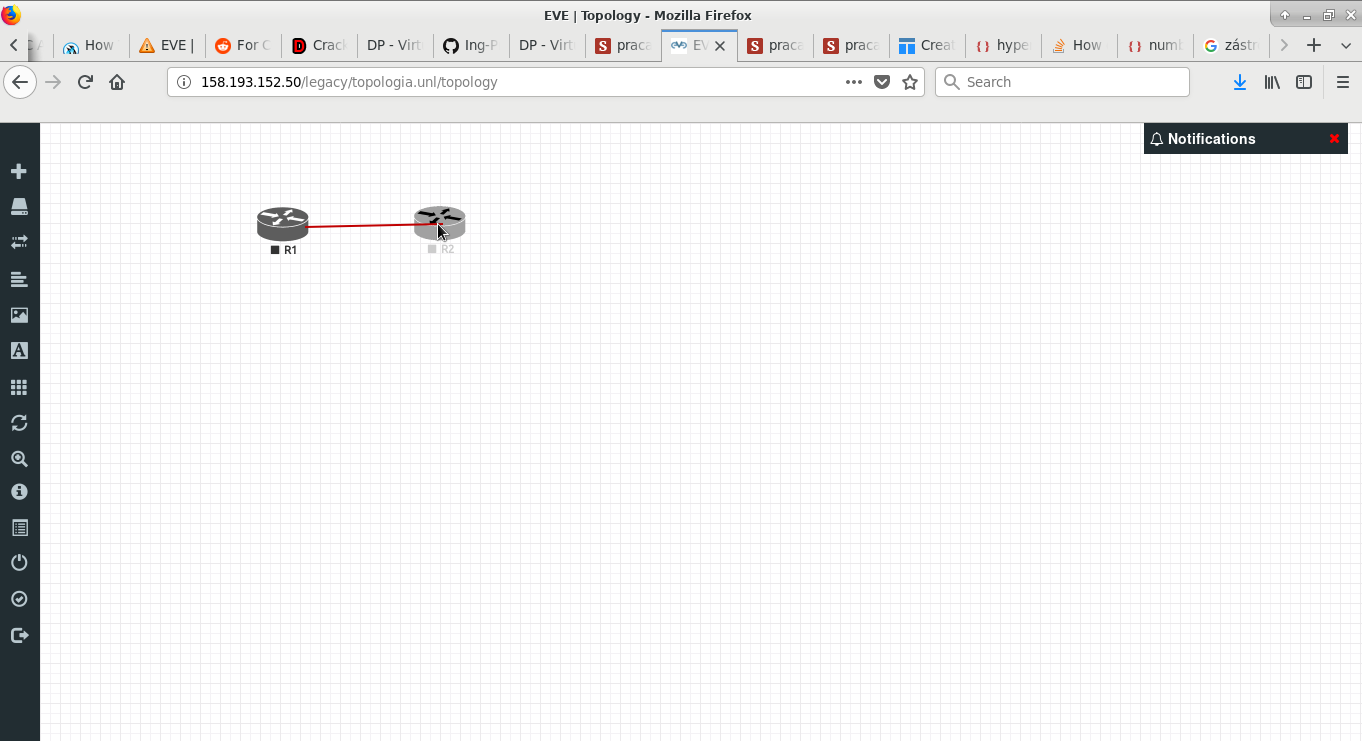
\includegraphics[width=0.75\textwidth]{eve_ng_prepajanie_ku_druhemu_zariadeniu}
        \caption{Priebeh prepájania zariadení}
        \label{obr:eve_ng_prepajanie_ku_druhemu_zariadeniu}
    \end{figure}
    
    \begin{figure}
        \centering
        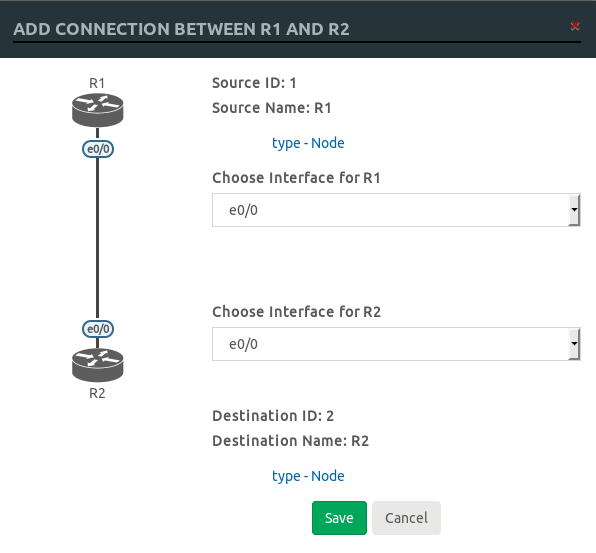
\includegraphics[width=0.75\textwidth]{eve_ng_prepajanie_add_connection_dialog}
        \caption{Dialógové okno na výber prepájaných rozhraní}
        \label{obr:eve_ng_prepajanie_add_connection_dialog}
    \end{figure}
    
    \begin{figure}
        \centering
        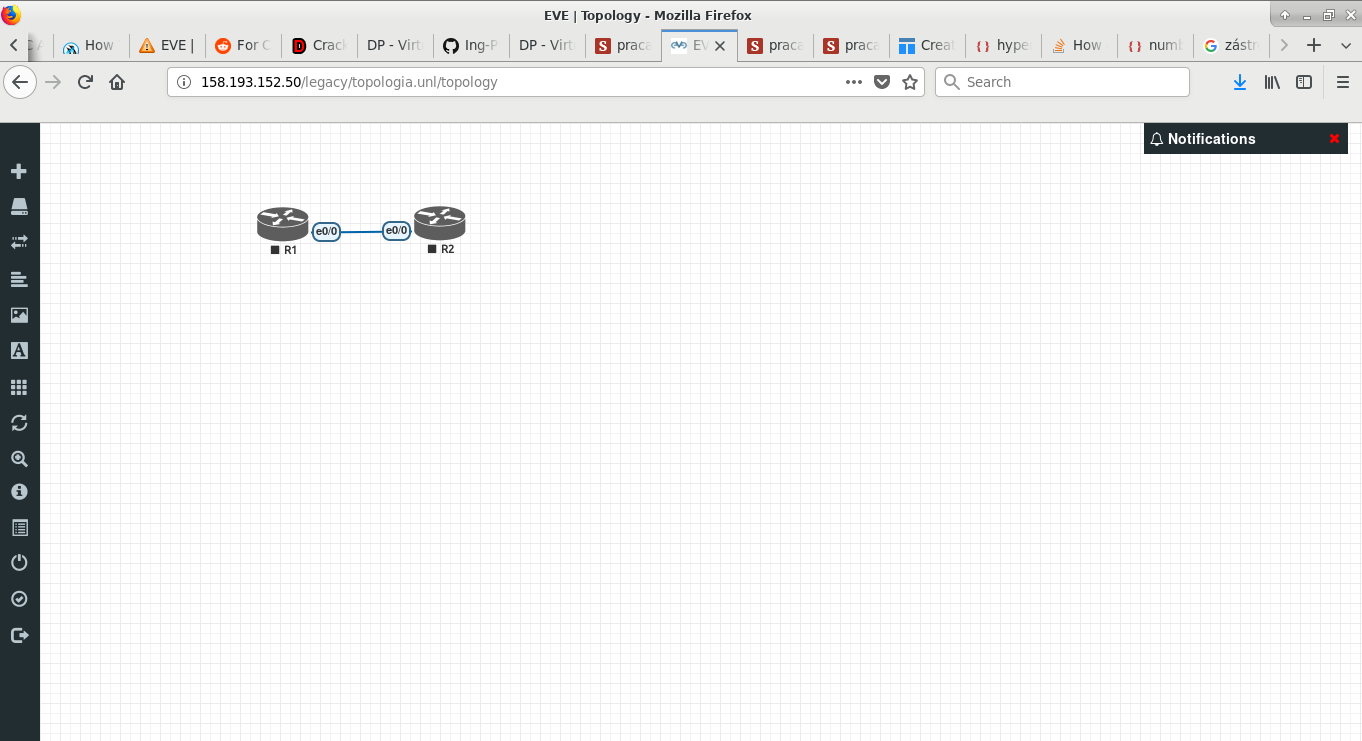
\includegraphics[width=0.75\textwidth]{eve_ng_prepajanie_prepojenie_vytvorenie}
        \caption{Úspešné vytvorenie prepojenia}
        \label{obr:eve_ng_prepajanie_prepojenie_vytvorenie}
    \end{figure}
    
    \item Po prepojení prvkov v topológii je možné upravovať ich atribúty rôznymi spôsobmi.
    
    \begin{itemize}[noitemsep]
        \item Najjednoduchším spôsobom úpravy platným pre všetky prvky je presunutie prvku myšou.
        \item Zariadenia je možné upravovať v zozname zariadení po kliknutí na položku \emph{Nodes} v menu na ľavej strane obrazovky (obr. \ref{obr:eve_ng_configured_nodes_dialog}).
        \item Ďalší spôsob, ako upraviť parametre zariadenia je pravým kliknutím na zariadenie a kliknutím na \emph{Edit} (obr. \ref{obr:eve_ng_edit_node_dialog}).
        \item Siete sa dajú upravovať v zozname sietí po kliknutí na položku \emph{Networks} v menu na ľavej strane obrazovky (obr. \ref{obr:eve_ng_configured_networks_dialog}).
        \item Obrázky, geometrické tvary a textové polia vieme upravovať v zozname objektov po kliknutí na položku \emph{Configured objects} v menu na ľavej strane obrazovky (obr. \ref{obr:eve_ng_configured_objects_dialog}).
    \end{itemize}

\begin{figure}
    \centering
    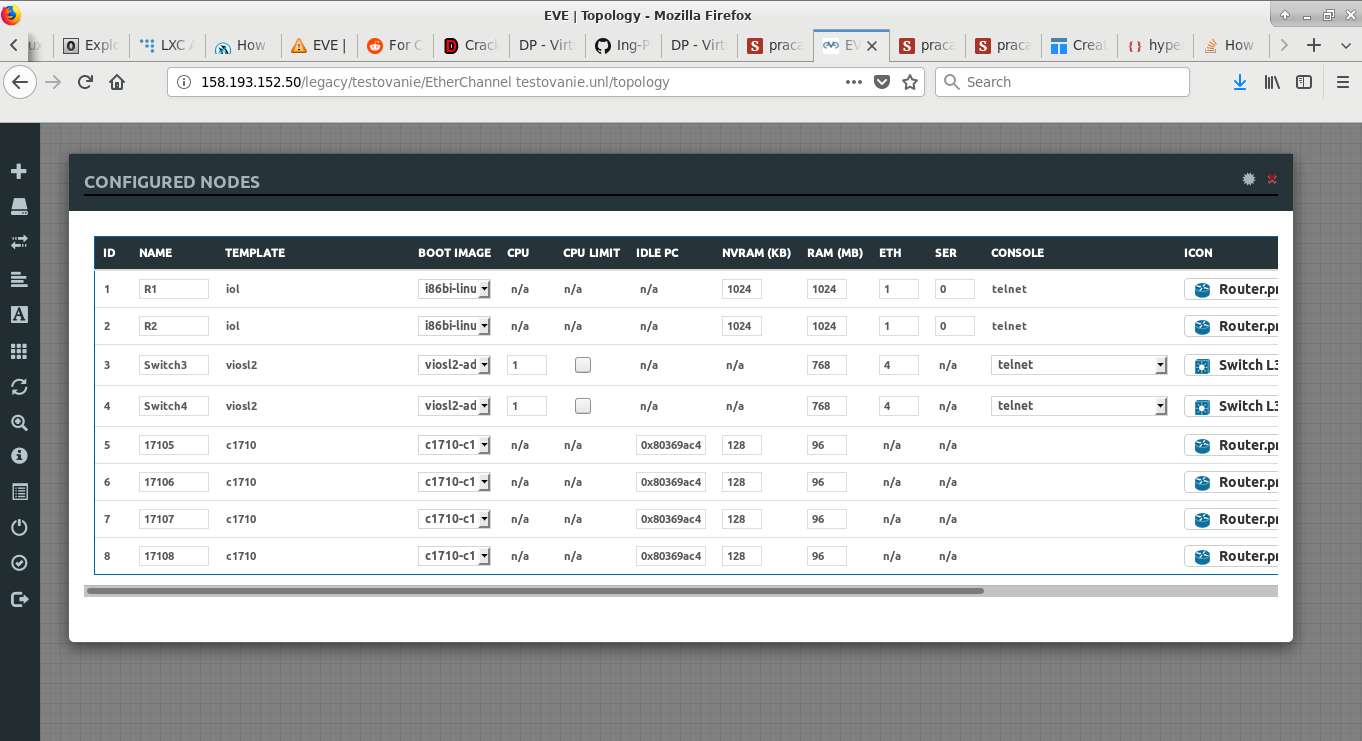
\includegraphics[width=0.75\textwidth]{eve_ng_configured_nodes_dialog}
    \caption{Dialógové okno so zoznamom zariadení v topológii}
    \label{obr:eve_ng_configured_nodes_dialog}
\end{figure}

\begin{figure}
    \centering
    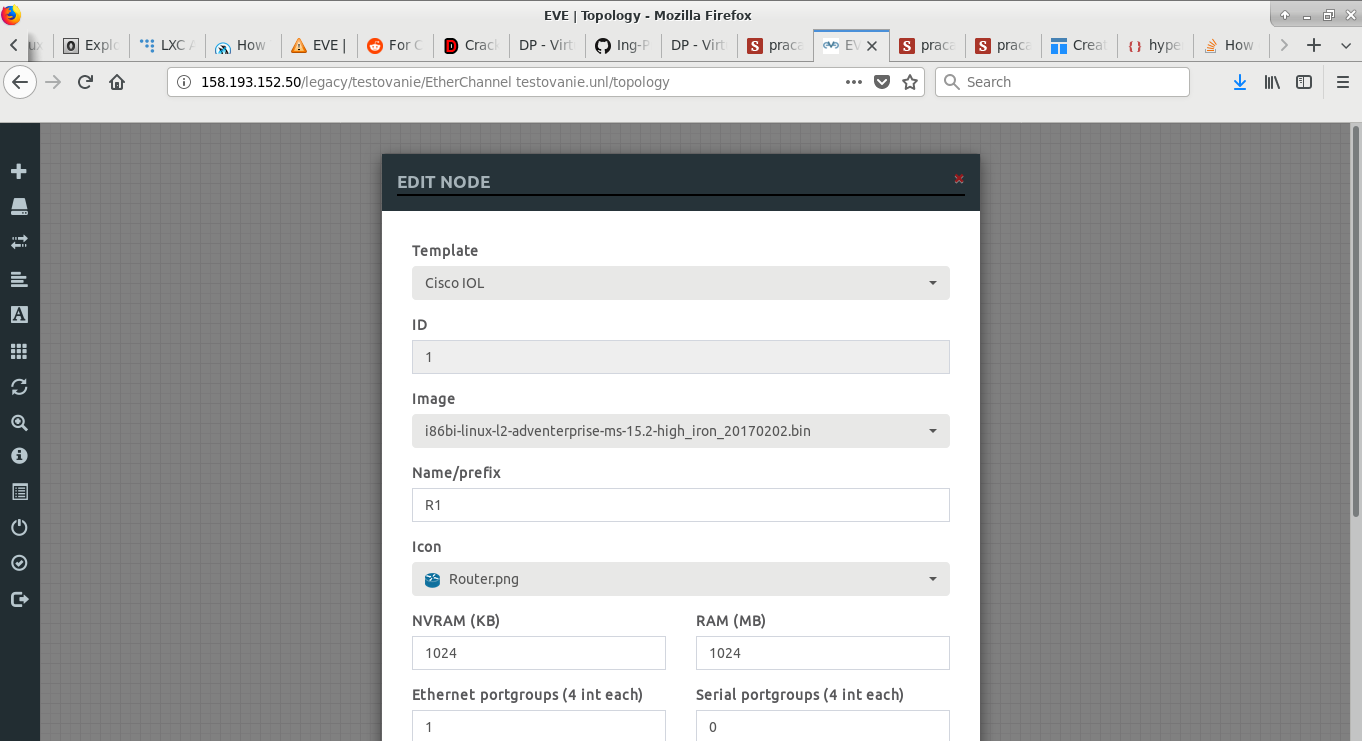
\includegraphics[width=0.75\textwidth]{eve_ng_edit_node_dialog}
    \caption{Dialógové okno na úpravu zariadenia}
    \label{obr:eve_ng_edit_node_dialog}
\end{figure}

\begin{figure}
    \centering
    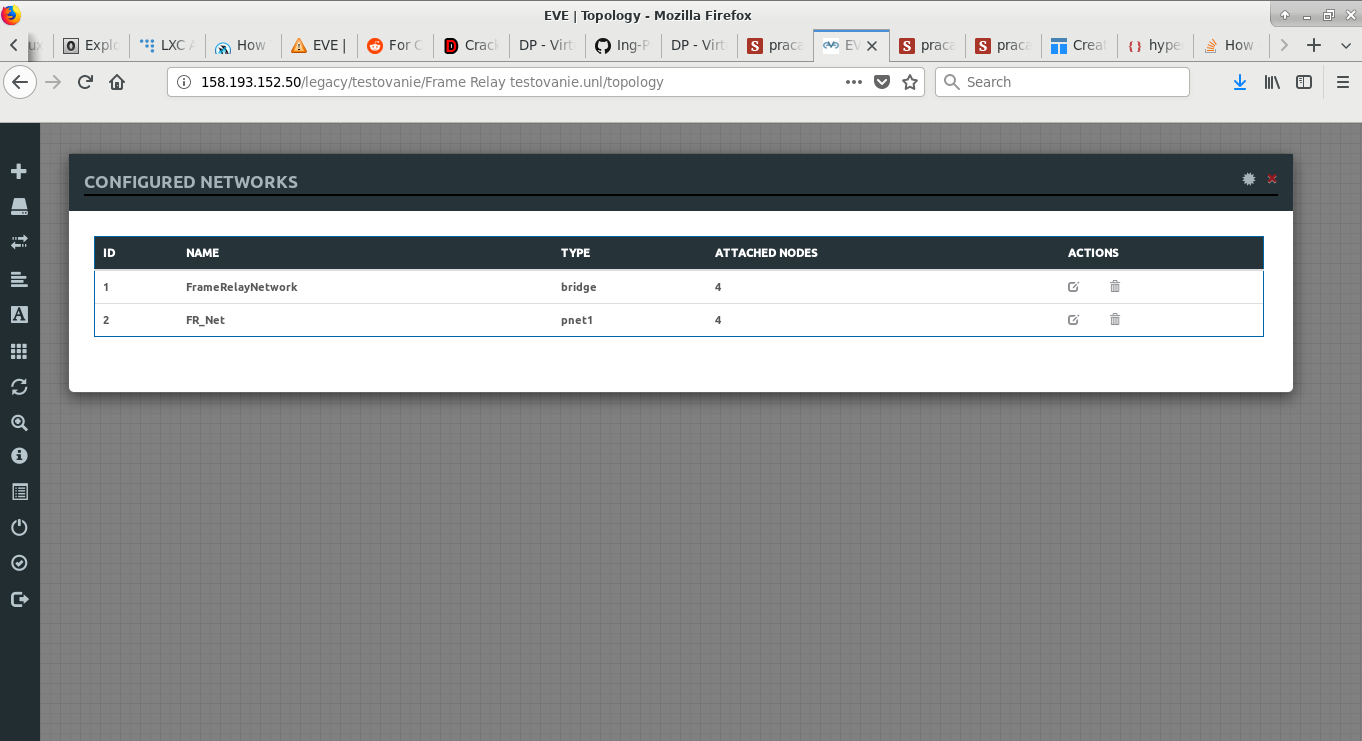
\includegraphics[width=0.75\textwidth]{eve_ng_configured_networks_dialog}
    \caption{Dialógové oknoso zoznamom sietí v topológii}
    \label{obr:eve_ng_configured_networks_dialog}
\end{figure}

\begin{figure}
    \centering
    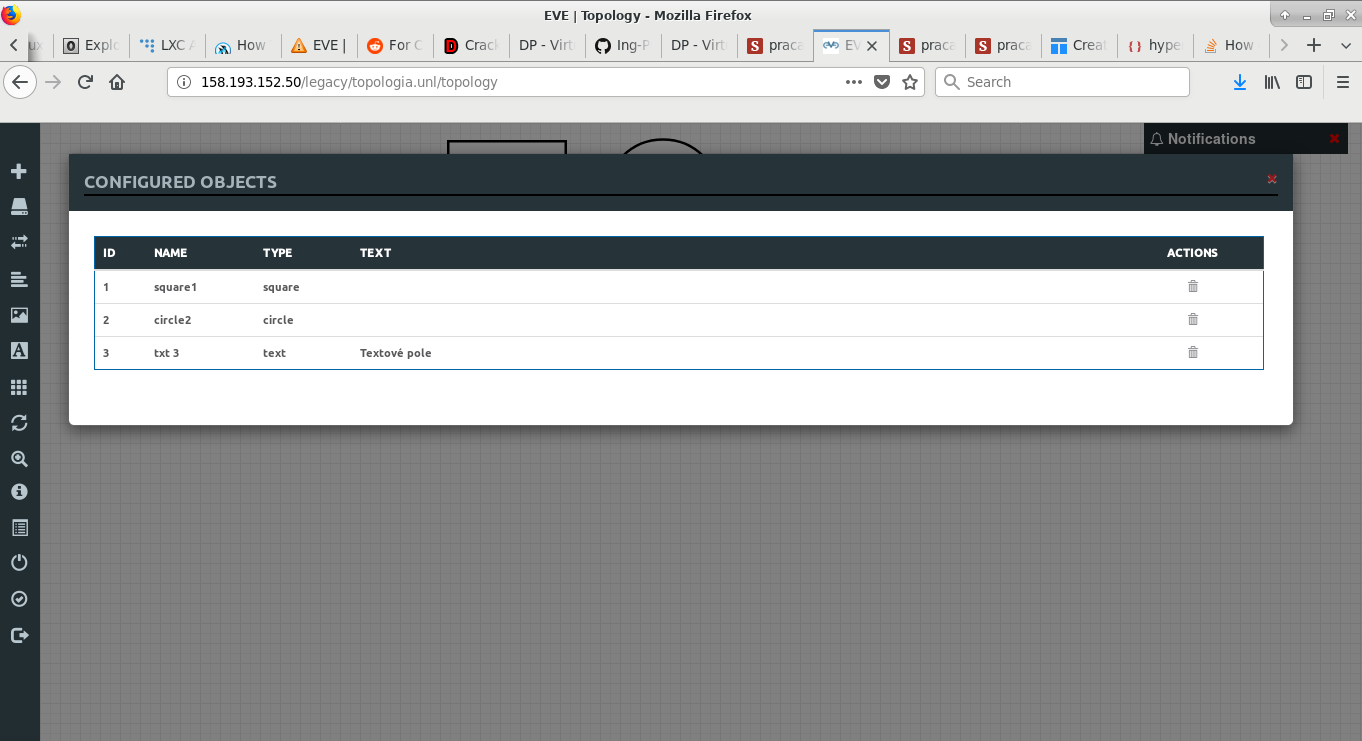
\includegraphics[width=0.75\textwidth]{eve_ng_configured_objects_dialog}
    \caption{Dialógové okno so zoznamom grafických a textových objektov}
    \label{obr:eve_ng_configured_objects_dialog}
\end{figure}



    
Ďalší spôsob na úpravu prvkov v topológii je pomocou upravením samotného súboru s topológiou na serveri s príponou \emph{unl} (obr. \ref{obr:eve_ng_unl_file_syntax}). Tento súbor je napísaný vo formáte XML. Prvky sú definované značkami, ktoré definujú ich typ (zariadenie, textové pole a pod.). Nižšie je uvedený zoznam niektorých značiek použitých v \emph{unl} súbore.

    \begin{description}[noitemsep]
        \item \textbf{\texttt{<node>}} - zariadenie v topológii
        \begin{description}[noitemsep]
            \item \textbf{\texttt{id}} - identifikačné číslo zariadenia; slúži na vygenerovanie portového čísla; musí byť unikátne
            \item \textbf{\texttt{name}} - názov zariadenia; zobrazuje sa pod jeho ikonkou; malo by byť unikátne, kvôli prehľadnosti topológie
            \item \textbf{\texttt{left}} - vzdialenosť od ľavého okraja plochy v topológii
            \item \textbf{\texttt{top}} - vzdialenosť od horného okraja plochy v topológii
            \item \textbf{\texttt{uuid}} - UUID identifikátor zariadenia; musí byť unikátny; iba pre QEMU zariadenia
            \item \textbf{\texttt{firstmac}} - MAC adresa prvého rohzrania pre zariadenia; iba pre QEMU zariadenia
            \item \textbf{\texttt{<interface>}} - pripojené rozhrania pre zariadenie
            \begin{description}[noitemsep]
                \item \textbf{\texttt{id}} - identifikačné číslo pripojeného rozhrania; musí byť unikátne
                \item \textbf{\texttt{remote\_id}} - identifikačné číslo vzdialeného zariadenia - odkaz na atribúť \texttt{id} v značke \texttt{<node>} iného zariadenia; iba pre IOL zariadenia
                \item \textbf{\texttt{network\_id}} - identifikačné číslo siete; iba pre Ethernet rozhrania 
            \end{description}
        \end{description}
        
        \item \textbf{\texttt{<networks>}} - zoznam vytvorených sietí v topológii
        \begin{description}[noitemsep]
            \item \textbf{\texttt{<network>}} - sieť v topológii; vytvára sa ako \emph{bridge} rozhranie pre prepojenie dvoch Ethernet rozhraní medzi zariadeniami
            \begin{description}[noitemsep]
                \item \textbf{\texttt{id}} - identifikačné číslo siete; musí byť unikátne
                \item \textbf{\texttt{visibility}} - viditeľnosť siete; v prípade, že prepájame dve Ethernet rohrania, je atribút nastavený na hodnotu 0 - sieť (bridge rozhranie) je v topológii skrytá. Ak pridávame do topológie sieť explicitne cez \emph{Add a new object} -> \emph{Network}, atribút sa nastaví na hodnotu 1 - sieť bude viditeľná v topológii.
            \end{description}
        \end{description}
    \end{description}

Zmeny v \emph{unl} súbore sa prejavia až po znovunačítaní stránky (klávesou F5) alebo topológie (kliknutím na \emph{Refresh topology} v menu na ľavej strane obrazovky).

\begin{figure}
    \centering
    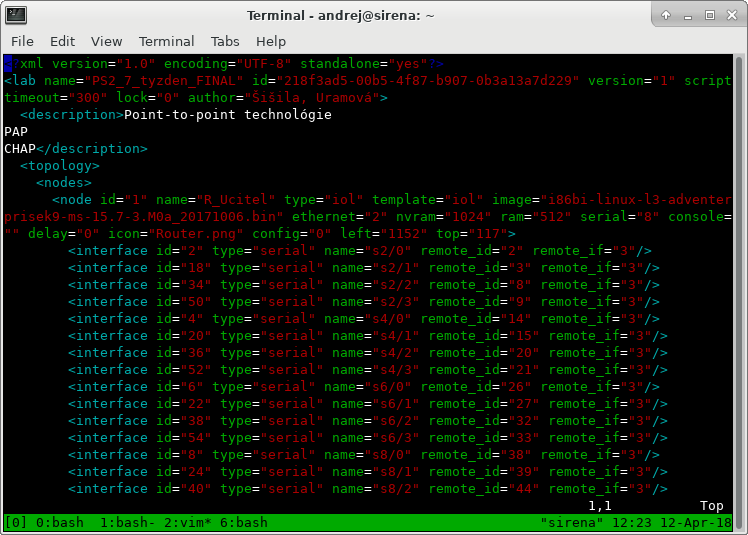
\includegraphics[width=0.75\textwidth]{eve_ng_unl_file_syntax}
    \caption{Ukážka UNL súboru}
    \label{obr:eve_ng_unl_file_syntax}
\end{figure}
    
Experimentovaním sme zistili, že vytváranie topológii a duplikácia jej prvkov v \emph{unl} súbore je pomerne náročná, zdĺhavá a náchylná na chyby. Pri duplikácii zariadení bolo náročné udržať prehľad o.i. aj o identifikátoroch zariadení a rozhraní a ich vzájomnom prepojení. Výhodnejšie sa ukázalo najprv použiť webové rozhranie, potom tabuľku zariadení \emph{Nodes} a nakoniec upravovať \emph{unl} súbor:
    
    \begin{enumerate}[noitemsep]
        \item Najpr vo webovom rozhraní vytvoríme topológiu, pridáme do nej zariadenia a poprepájame ich.
        \item Potom v tabuľke zariadeníNodes (nazvy zariadeni)
        \item Ak je potrebné, nakoniec v \emph{unl} súbore presnejšie upravíme súradnice prvkov v topológii definovaných atribútmi \texttt{left} a \texttt{top}. Výsledkom týchto úprav je celkové zlepšenie estetickej úpravy. Môžeme tak urobiť aj vo webovom rozhraní v dialógovom okne pre úpravu zariadenia v atribútoch \emph{Left} a \emph{Top}, avšak v \emph{unl} súbore vieme súradnice prvkov upraviť hromadne.
    \end{enumerate}
    
    \item Potom, ako sme pridali zariadenia do topológie a navzájom ich prepojili, môžeme zariadenia spustiť buď jednotlivo, skupinovo alebo všetky naraz. Zariadenia môže spúšťať iba používateľ s rolou \emph{admin} alebo \emph{editor}.

    \begin{itemize}[noitemsep]
        \item Jedno zariadenie spustíme tak, že naň klikneme pravým tlačidlom a zvolíme \emph{Start} (obr. \ref{obr:eve_ng_spustanie_po_jednom_context_menu}).
        \item Skupinu zariadení spustíme tak, že ich najpr označíme myšou resp. vyberieme zariadenia kombináciou \emph{Ctrl + ľavé kliknutie}. Následne na jedno z označených zariadení klikneme pravým tlačidlom a zvolíme \emph{Start Selected} (obr. \ref{obr:eve_ng_spustanie_skupiny_context_menu}).
        \item Všetky zariadenia spustíme kliknutím na položku \emph{More actions} a zvolíme možnosť \emph{Start all nodes} (obr. \ref{obr:eve_ng_spustanie_vsetkych_context_menu}).
    \end{itemize}

\begin{figure}
    \centering
    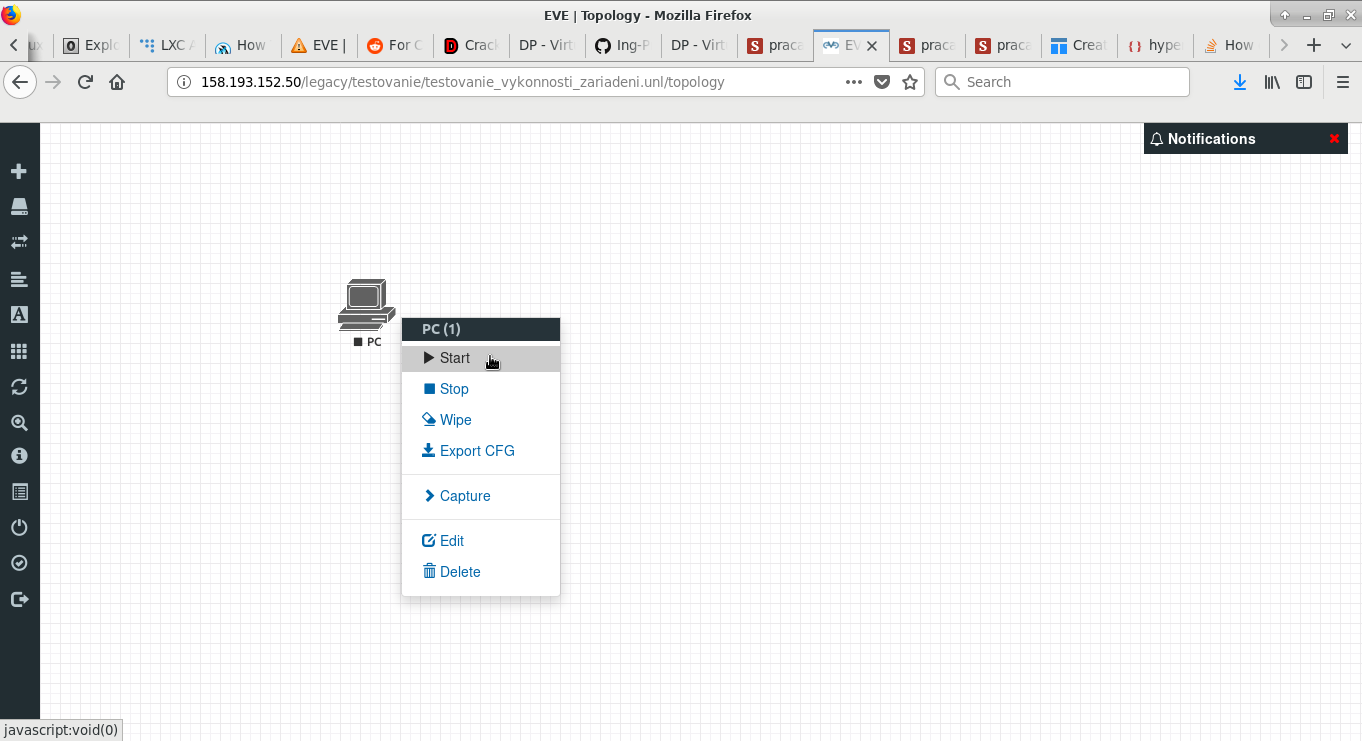
\includegraphics[width=0.75\textwidth]{eve_ng_spustanie_po_jednom_context_menu}
    \caption{Spustenie jedného zariadenia}
    \label{obr:eve_ng_spustanie_po_jednom_context_menu}
\end{figure}

\begin{figure}
    \centering
    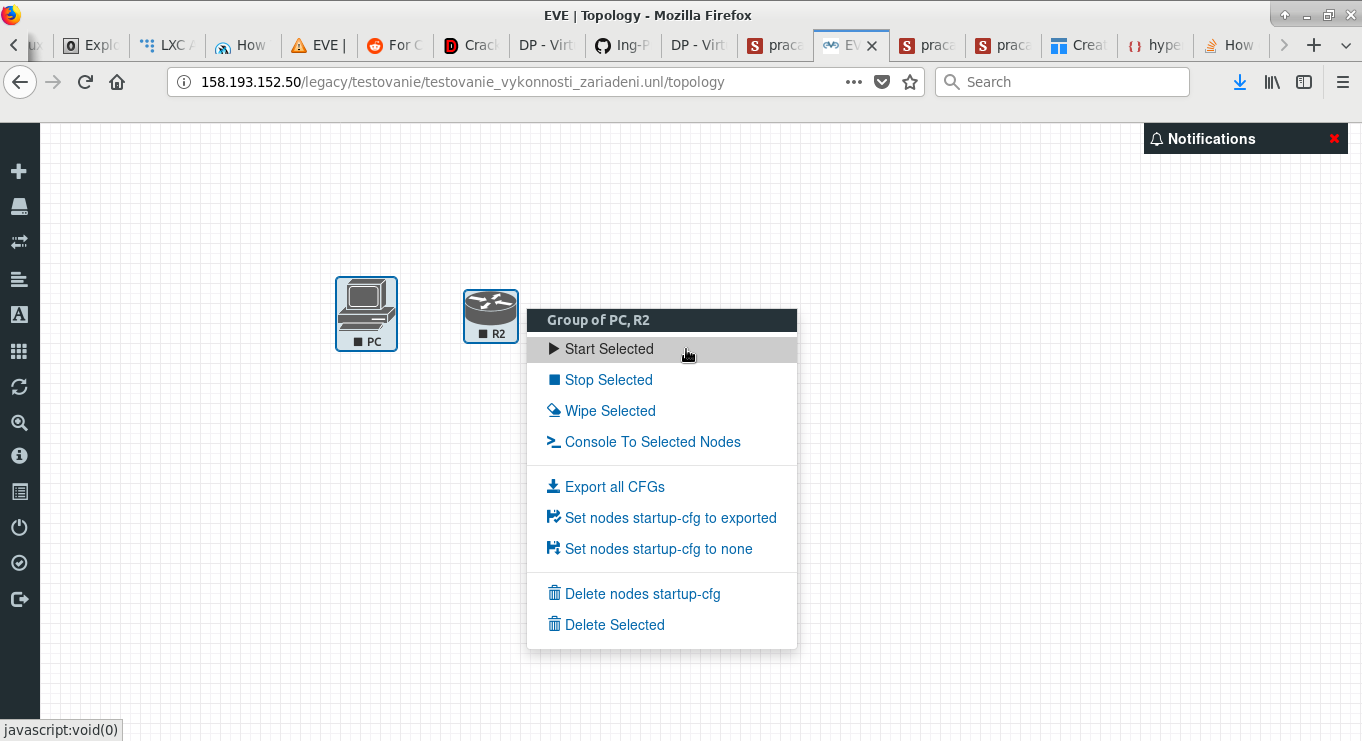
\includegraphics[width=0.75\textwidth]{eve_ng_spustanie_skupiny_context_menu}
    \caption{Spustenie skupiny zariadení}
    \label{obr:eve_ng_spustanie_skupiny_context_menu}
\end{figure}

\begin{figure}
    \centering
    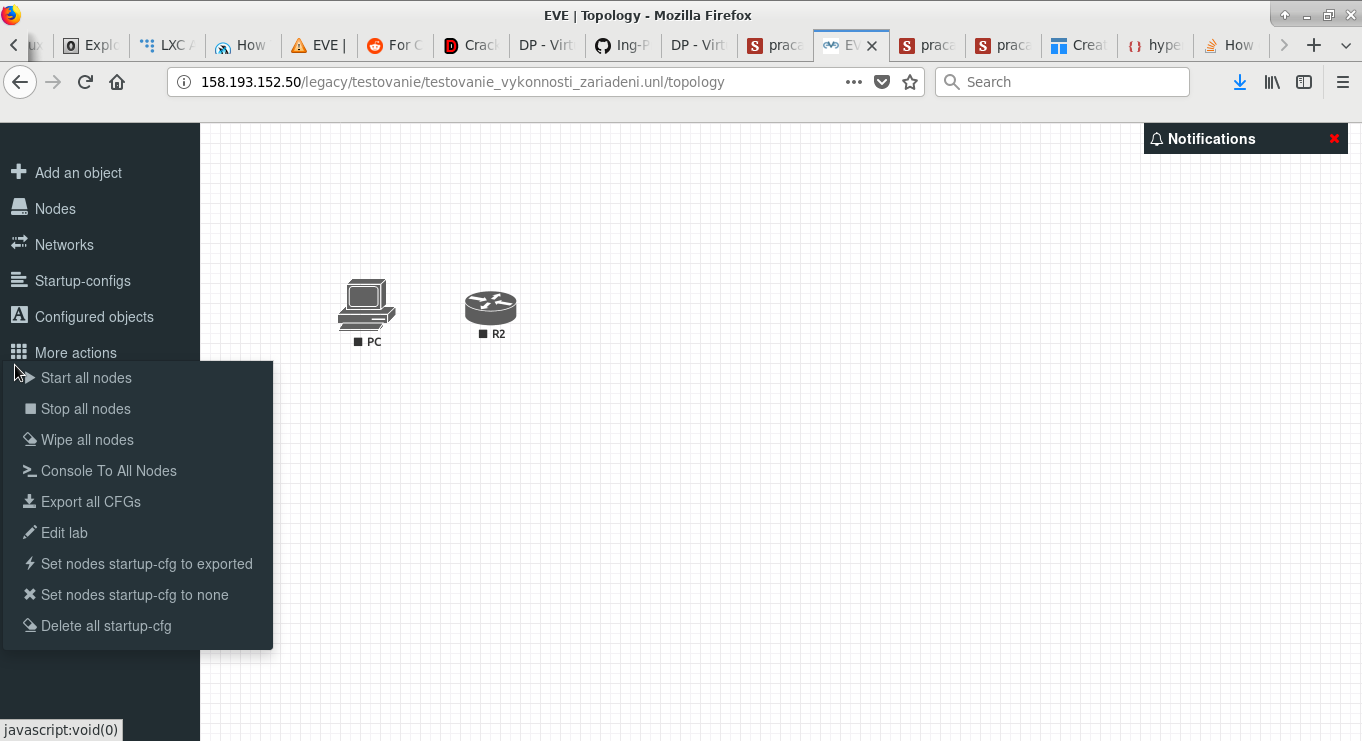
\includegraphics[width=0.75\textwidth]{eve_ng_spustanie_vsetkych_sidemenu}
    \caption{Spustenie všetkých zariadení}
    \label{obr:eve_ng_spustanie_vsetkych_context_menu}
\end{figure}
      
    \item \label{item:vzdialeny_pristup} Po spustení zariadení je možné pripojiť sa na ich vzdialenú konzolu. Spôsob, akým sa na pripájame na konzoly zariadení sa líši podľa toho, v akom móde sme sa do EVE-ng prihlásili. V bode \ref{item:prihlasenie} sme spomenuli, že do webového rozhrania EVE-ng je možné sa prihlásiť v dvoch módoch: HTML5 a natívnom móde. Výber módu priamo ovplyvňuje aj spôsob, akým pristupujeme ku konzolám zariadení.
    
    HTML5 mód zabezpečuje vzdialený prístup k zariadeniam pomocou reverzného proxy servera \emph{Apache Guacamole}, ktorý sa pripája na konzoly zariadení. VV tomto móde sa na obrazovke s otvorenou topológiou po kliknutí na zariadenie otvorí jeho vzdialená konzola, pričom nie je možné pripojiť sa ku konzolám zariadenia pomocou telnet alebo vnc klienta. HTML5 mód web rozhrania EVE-ng bol však menej stabilný a reagoval výrazne pomalšie pri práci s topológiou v provonaní s natívnym módom. Preto bolo webové rozhranie ďalej používané iba v natívnom móde.
        
    V natívnom móde potrebujeme mať pre vzdialený prístup ku zariadeniam nainštalované dodatočné nástroje na lokálnom počítači. 
        
    Na prístup k zariadeniam z lokálneho počítača potrebujeme mať nainštalovaného telnet a VNC klienta. Pre platformu Windows môžeme zvoliť kombináciu napr. \emph{PuTTY} a \emph{RealVNC Viewer}, pre platformu Linux zase terminál (odporúča sa BASH) a \emph{TigerVNC}. Následne sa navigujeme myšou na zariadenie, na ktoré sa chceme pripojiť, ale namiesto toho, aby sme naň klikli, zapamätáme si údaje zobrazené v ľavom alebo pravom dolnom rohu obrazovky (obr. \ref{obr:eve_ng_protokol_ip_port}) t.j. protokol, IP adresa servera a portové číslo. Tieto údaje následne zadáme do zodpovedajúceho klienta podľa protokolu. Po zadaní správnych údajov by sme sa mali pripojiť na vzdialenú konzolu zariadenia.

\begin{figure}
    \centering
    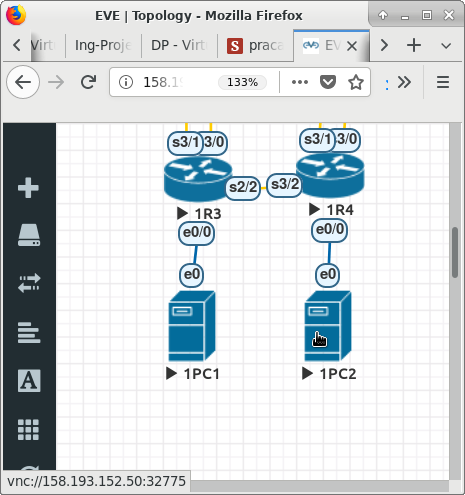
\includegraphics[width=0.75\textwidth]{eve_ng_protokol_ip_port}
    \caption{Adresa na vzdialený prístup k zariadeniu}
    \label{obr:eve_ng_protokol_ip_port}
\end{figure}

    Aby sme mohli pristupovať ku konzole zariadenia z webového rozhrania pri kliknutí naň, potrebujeme mať na lokálnom počítači nainštalovaný tzv. EVE-ng integračný balíček. Ten existuje pre platformy Windows a Linux. Ďalej sme upravovali iba integračný balíček pre platformu Linux, z ktorého nakoniec vznikla ďalšia, bezpečnejšia verzia. Jednalo sa úpravy, ktoré zabezpečovali vzdialený prístup k zariadeniam s protokolmi \emph{telnet} a \emph{vnc} pomocou SSH tunelov a odchytávanie prevádzky z rozhrania zariadenia ako štandardný používateľ namiesto používateľa \emph{root}. Predvolený integračný baliček takéto funkciu neobsahuje. Vykonané úpravy nemajú výrazný vplyv na funkcionalitu pre koncového používateľa. Inštalácia a úprava integračného balíčka EVE-ng pre platformy Windows a Linux je popísaná v súbore na CD s názvom \\
    \emph{eve\_ng/16\_0\_eve-ng\_integracia\_s\_web\_prehliadacmi.txt}.

\end{enumerate}

Vyššie uvedené kroky popisujú vytvorenie základnej topológie s rôznymi prvkami. V ďalších častiach bude popísané, ako EVE-ng generuje a priďeľuje portové čísla zariadeniam, pomocou ktorých sa pripájame na ich vzdialené konzoly a to, ako prepojiť viacero topológii medzi sebou, a ako pripojiť topológiu k internetu.




\subsection{Prideľovanie portových čísel zariadeniam}
\label{chap:priradovanie_portovych_cisel}

Po pridaní ľubovoľného zariadenia do topológie sa preň vygeneruje portové číslo, ktoré mu je následne priradené. Portové čísla rozlišujú zariadenia v topológii a  slúžia na pripojenie sa na ich vzdialené konzoly. Vždy sa vyberie najnižšie dostupné portové číslo.

Rozsah portových čísel pre daného používateľa sa generujú vzťahom \emph{32768 + 128 * POD + ID}, kde \emph{POD} je unikátne identifikačné číslo používateľa a \emph{ID} je unikátne identifikačné číslo zariadenia. Za uvedený výpočet je zodpovená funkcia \texttt{\_\_construct} v súbore \\ \emph{/opt/unetlab/html/includes/\_\_node.php}.

Ak do topológie pridáme viacero zariadení naraz, budú mať portové čísla idúce za sebou.

V prípade, že si rôzni používatelia otvoria rovnaký súbor s topológiou, bude mať každý z používateľov prístup ku vlastným zariadeniam. Pokiaľ bude počet zariadení v topológii <= 63, portové čísla zariadení sa nebudú prekrývať a každý z používateľov bude môcť pracovať s topológiou nezávisle na sebe. Ak ľubovoľný z používateľov do topológie pridá zariadenie, uvidia ho všetci.

Vyššie uvedené správanie bolo otestované po otvorení rovnakého súboru s topológiou dvomi rôznymi používateľmi s rôznymi používateľskými rolami (\emph{admin} a \emph{editor}). Na obr. \ref{obr:eve_ng_rovnaka_topo_prvy_pouzivatel_admin} vidíme, že prvý používateľ už má spustené zariadenia, ale druhý používateľ ich ako spustené nevidí (obr. \ref{obr:eve_ng_rovnaka_topo_druhy_pouzivatel_editor}).

\begin{figure}
    \centering
    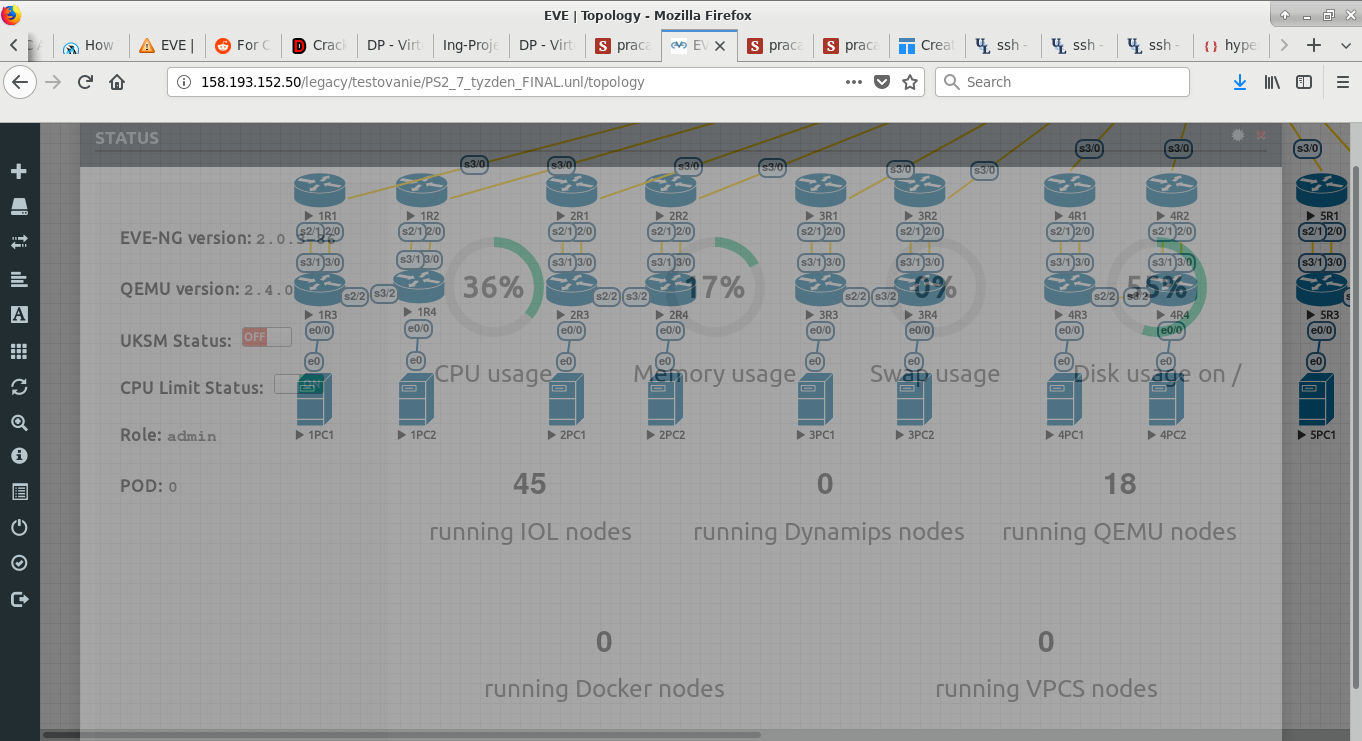
\includegraphics[width=0.75\textwidth]{eve_ng_rovnaka_topo_prvy_pouzivatel_admin}
    \caption{Topológia prvého používateľa s používateľskou rolou \emph{admin}}
    \label{obr:eve_ng_rovnaka_topo_prvy_pouzivatel_admin}
\end{figure}

\begin{figure}
    \centering
    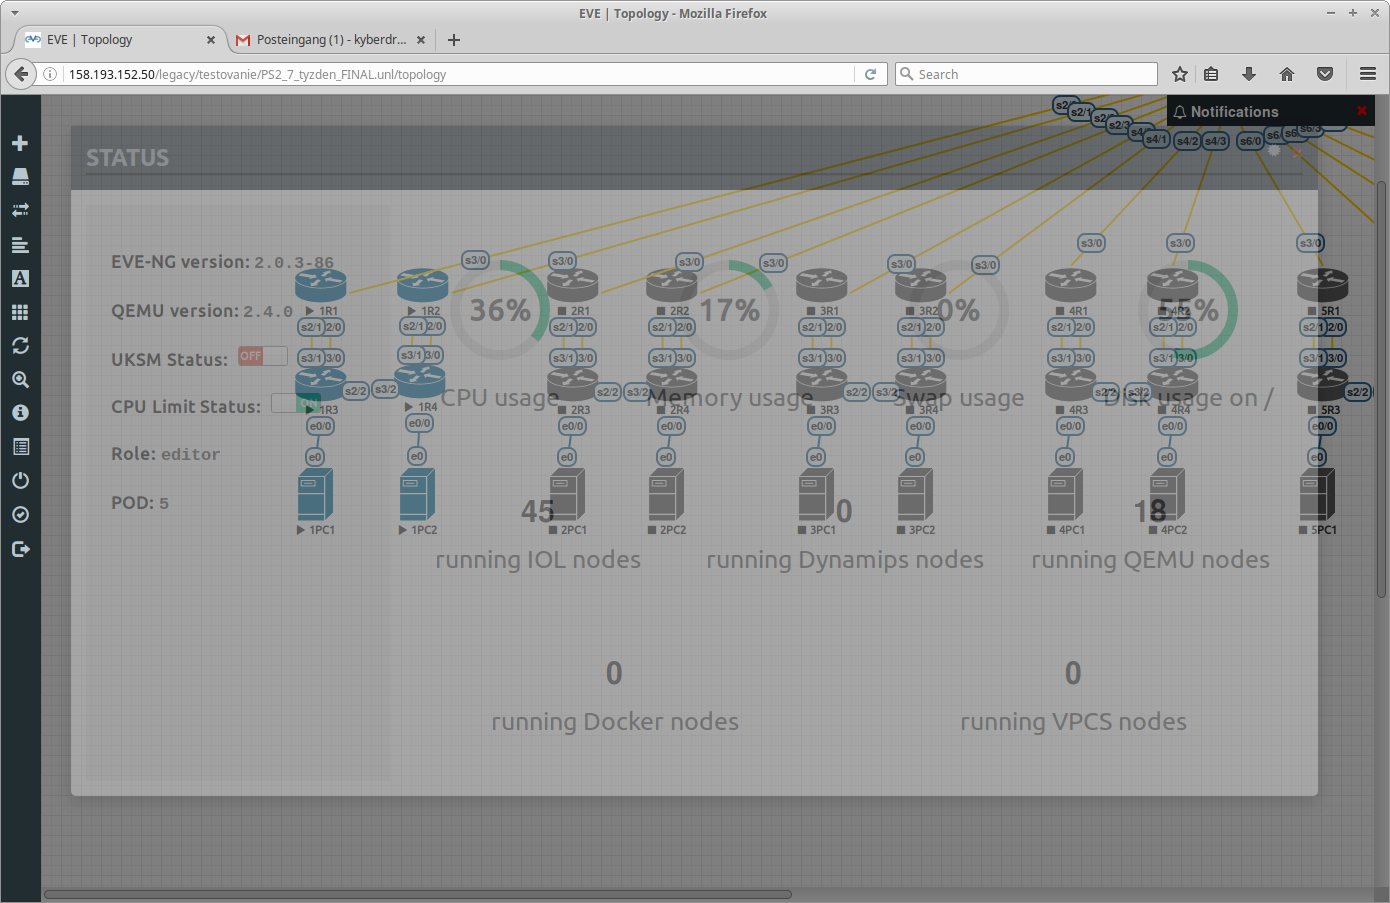
\includegraphics[width=0.75\textwidth]{eve_ng_rovnaka_topo_druhy_pouzivatel_editor}
    \caption{Topológia druhého používateľa s používateľskou rolou \emph{editor}}
    \label{obr:eve_ng_rovnaka_topo_druhy_pouzivatel_editor}
\end{figure}





\subsection{Pripojenie topológie k internetu / prepojenie topológii navzájom}

Do EVE-ng topológie je možné pridať prvok typu \emph{sieť}, ktorý umožňuje prepájať topológie medzi sebou alebo ich pripájať ku internetu.

Sieť do topológie pridáme kliknutím na ikonu \emph{+ - Add an object} a zo zoznamu vybierieme položku \emph{Network}. Objaví sa dialógové okno na úpravu parametrov pridávanej siete (obr. \ref{obr:eve_ng_add_network_dialog}). Pre správnu funkčnosť a prehľadnosť stačí zmeniť iba atribúty \emph{Name} a \emph{Type}. To textového poľa atribútu \emph{Name} zadáme názov pridávanej siete. Z rozbaľovacieho zoznamu (obr. \ref{obr:eve_ng_add_network_dialog_network_types}) si následne zvolíme typ siete:

\begin{figure}
    \centering
    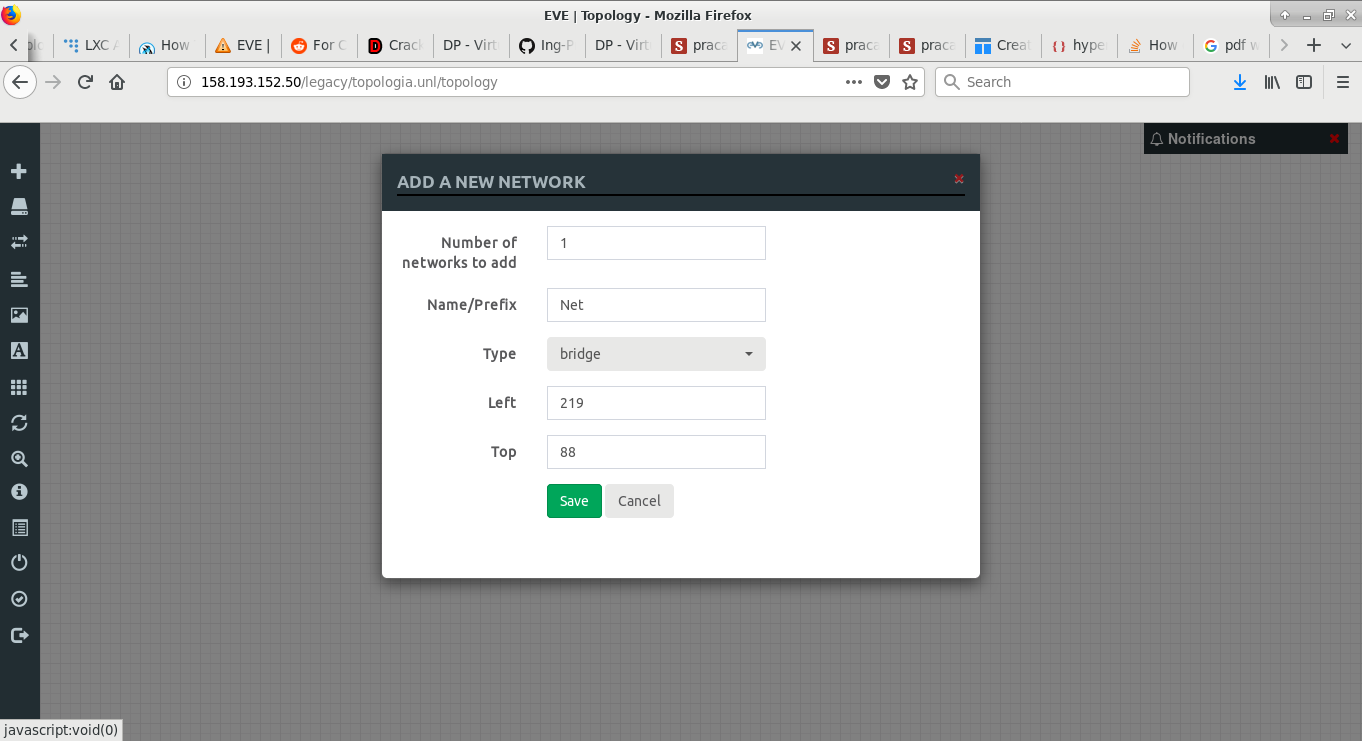
\includegraphics[width=0.75\textwidth]{eve_ng_add_network_dialog}
    \caption{Dialógové okno pre pridanie siete}
    \label{obr:eve_ng_add_network_dialog}
\end{figure}

\begin{description}
    \item \textbf{bridge} - Slúži na vytvorenie siete na prepojenie zariadení v jednej topológii.
    \item \textbf{Management (Cloud0)} - Sieť, pomocou ktorj vieme pripojiť topológiu k živej sieti alebo internetu.
    \item \textbf{Cloud1-9} - Siete, ktoré slúžia na prepájanie topológii medzi sebou na jednom serveri.
\end{description}

\begin{figure}
    \centering
    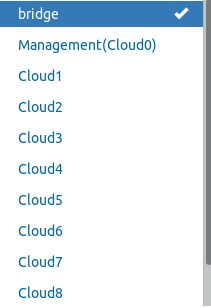
\includegraphics[width=0.75\textwidth]{eve_ng_add_network_dialog_network_types}
    \caption{Typy sietí}
    \label{obr:eve_ng_add_network_dialog_network_types}
\end{figure}

Po pridaní siete do topológie k nej môžeme pripájať ľubovoľný počet zariadení prostredníctvom Ethernet rozhraní. Sieť bude pre zariadenia pripojené na sieť slúžiť ako \emph{hub (rozdeľovač)}.

V prípade, že topológiu pripájame na živú sieť prostredníctvom \emph{Cloud0}, je potrebné pre rozhranie zariadenia pripojeného k tejto sieti priradiť IP adresu buď pomocou DHCP, alebo staticky manuálnou konfiguráciou. Ak je potrebné, povolíme IP adresu na zariadení \emph{firewall}. Príklad topológie s rôznymi typmi sietí je znázornený na obr. \ref{obr:eve_ng_siete_v_topologii}.

\begin{figure}
    \centering
    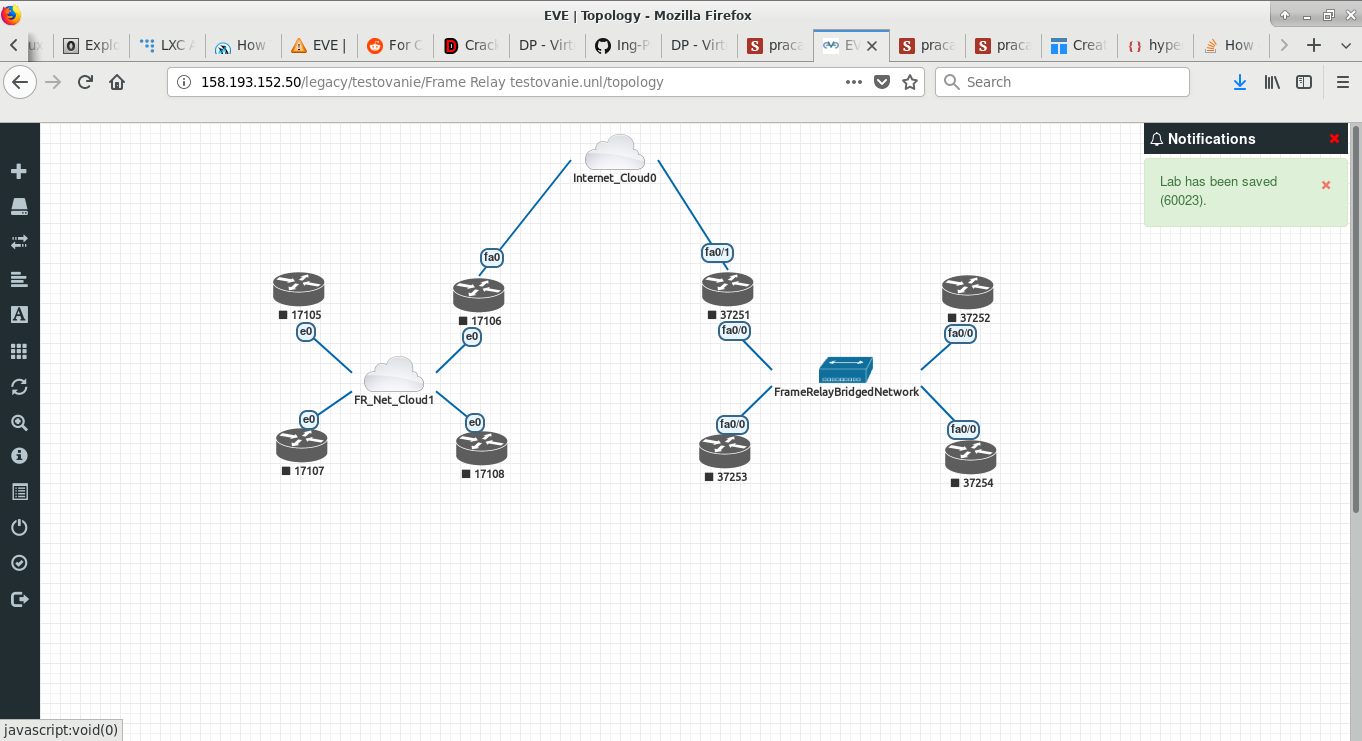
\includegraphics[width=0.75\textwidth]{eve_ng_siete_v_topologii}
    \caption{Ukážka topológie s rôznymi typmi sietí}
    \label{obr:eve_ng_siete_v_topologii}
\end{figure}